\documentclass[twoside]{book}

% Packages required by doxygen
\usepackage{fixltx2e}
\usepackage{calc}
\usepackage{doxygen}
\usepackage[export]{adjustbox} % also loads graphicx
\usepackage{graphicx}
\usepackage[utf8]{inputenc}
\usepackage{makeidx}
\usepackage{multicol}
\usepackage{multirow}
\PassOptionsToPackage{warn}{textcomp}
\usepackage{textcomp}
\usepackage[nointegrals]{wasysym}
\usepackage[table]{xcolor}

% Font selection
\usepackage[T1]{fontenc}
\usepackage[scaled=.90]{helvet}
\usepackage{courier}
\usepackage{amssymb}
\usepackage{sectsty}
\renewcommand{\familydefault}{\sfdefault}
\allsectionsfont{%
  \fontseries{bc}\selectfont%
  \color{darkgray}%
}
\renewcommand{\DoxyLabelFont}{%
  \fontseries{bc}\selectfont%
  \color{darkgray}%
}
\newcommand{\+}{\discretionary{\mbox{\scriptsize$\hookleftarrow$}}{}{}}

% Page & text layout
\usepackage{geometry}
\geometry{%
  a4paper,%
  top=2.5cm,%
  bottom=2.5cm,%
  left=2.5cm,%
  right=2.5cm%
}
\tolerance=750
\hfuzz=15pt
\hbadness=750
\setlength{\emergencystretch}{15pt}
\setlength{\parindent}{0cm}
\setlength{\parskip}{3ex plus 2ex minus 2ex}
\makeatletter
\renewcommand{\paragraph}{%
  \@startsection{paragraph}{4}{0ex}{-1.0ex}{1.0ex}{%
    \normalfont\normalsize\bfseries\SS@parafont%
  }%
}
\renewcommand{\subparagraph}{%
  \@startsection{subparagraph}{5}{0ex}{-1.0ex}{1.0ex}{%
    \normalfont\normalsize\bfseries\SS@subparafont%
  }%
}
\makeatother

% Headers & footers
\usepackage{fancyhdr}
\pagestyle{fancyplain}
\fancyhead[LE]{\fancyplain{}{\bfseries\thepage}}
\fancyhead[CE]{\fancyplain{}{}}
\fancyhead[RE]{\fancyplain{}{\bfseries\leftmark}}
\fancyhead[LO]{\fancyplain{}{\bfseries\rightmark}}
\fancyhead[CO]{\fancyplain{}{}}
\fancyhead[RO]{\fancyplain{}{\bfseries\thepage}}
\fancyfoot[LE]{\fancyplain{}{}}
\fancyfoot[CE]{\fancyplain{}{}}
\fancyfoot[RE]{\fancyplain{}{\bfseries\scriptsize Generated by Doxygen }}
\fancyfoot[LO]{\fancyplain{}{\bfseries\scriptsize Generated by Doxygen }}
\fancyfoot[CO]{\fancyplain{}{}}
\fancyfoot[RO]{\fancyplain{}{}}
\renewcommand{\footrulewidth}{0.4pt}
\renewcommand{\chaptermark}[1]{%
  \markboth{#1}{}%
}
\renewcommand{\sectionmark}[1]{%
  \markright{\thesection\ #1}%
}

% Indices & bibliography
\usepackage{natbib}
\usepackage[titles]{tocloft}
\setcounter{tocdepth}{3}
\setcounter{secnumdepth}{5}
\makeindex

% Custom commands
\newcommand{\clearemptydoublepage}{%
  \newpage{\pagestyle{empty}\cleardoublepage}%
}

\usepackage{caption}
\captionsetup{labelsep=space,justification=centering,font={bf},singlelinecheck=off,skip=4pt,position=top}

%===== C O N T E N T S =====

\begin{document}

% Titlepage & ToC
\pagenumbering{roman}
\begin{titlepage}
\vspace*{7cm}
\begin{center}%
{\Large Assignment5 }\\
\vspace*{1cm}
{\large Generated by Doxygen 1.8.11}\\
\end{center}
\end{titlepage}
\clearemptydoublepage
\tableofcontents
\clearemptydoublepage
\pagenumbering{arabic}

%--- Begin generated contents ---
\chapter{Hierarchical Index}
\section{Class Hierarchy}
This inheritance list is sorted roughly, but not completely, alphabetically\+:\begin{DoxyCompactList}
\item \contentsline{section}{General\+Number}{\pageref{classGeneralNumber}}{}
\begin{DoxyCompactList}
\item \contentsline{section}{General\+Double}{\pageref{classGeneralDouble}}{}
\item \contentsline{section}{General\+Long}{\pageref{classGeneralLong}}{}
\item \contentsline{section}{General\+Rational}{\pageref{classGeneralRational}}{}
\end{DoxyCompactList}
\end{DoxyCompactList}

\chapter{Class Index}
\section{Class List}
Here are the classes, structs, unions and interfaces with brief descriptions\+:\begin{DoxyCompactList}
\item\contentsline{section}{{\bf Foo} }{\pageref{classFoo}}{}
\item\contentsline{section}{{\bf Stack} }{\pageref{classStack}}{}
\end{DoxyCompactList}

\chapter{File Index}
\section{File List}
Here is a list of all files with brief descriptions\+:\begin{DoxyCompactList}
\item\contentsline{section}{{\bf calc.\+cpp} }{\pageref{calc_8cpp}}{}
\item\contentsline{section}{{\bf General\+Number.\+cpp} }{\pageref{GeneralNumber_8cpp}}{}
\item\contentsline{section}{{\bf General\+Number.\+h} }{\pageref{GeneralNumber_8h}}{}
\item\contentsline{section}{{\bf gnparse.\+cpp} }{\pageref{gnparse_8cpp}}{}
\item\contentsline{section}{{\bf gntest.\+cpp} }{\pageref{gntest_8cpp}}{}
\end{DoxyCompactList}

\chapter{Class Documentation}
\section{General\+Double Class Reference}
\label{classGeneralDouble}\index{General\+Double@{General\+Double}}


{\ttfamily \#include $<$General\+Number.\+h$>$}

Inheritance diagram for General\+Double\+:\begin{figure}[H]
\begin{center}
\leavevmode
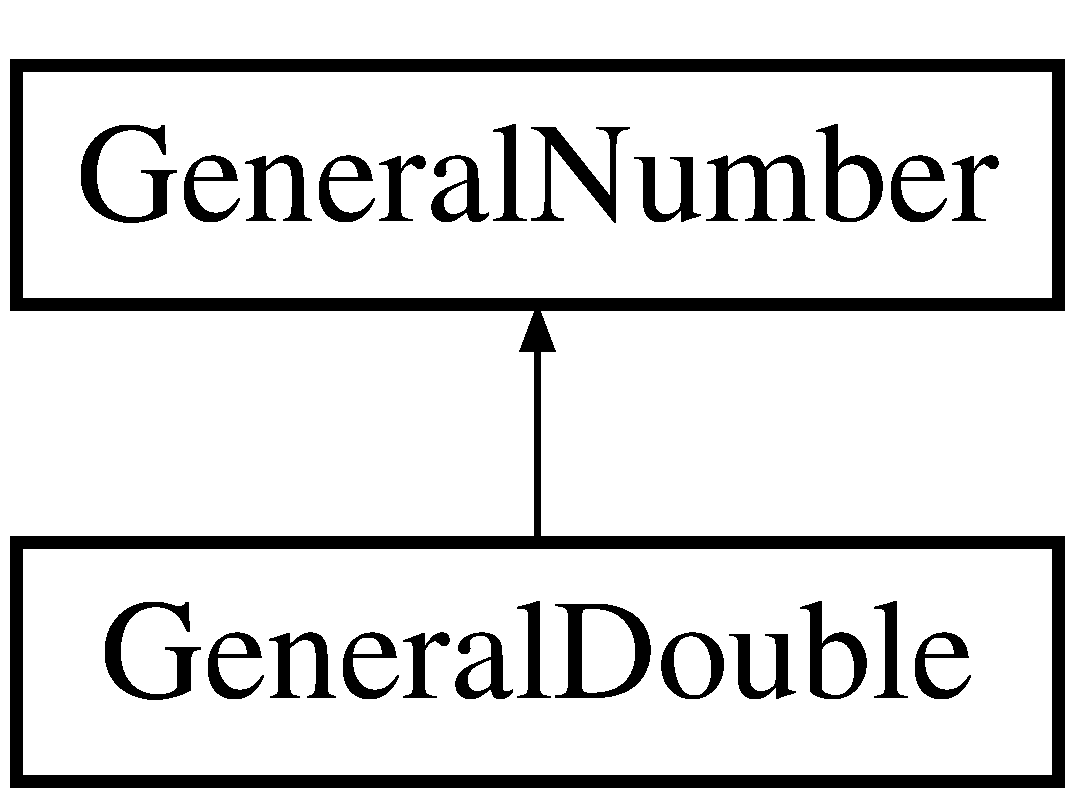
\includegraphics[height=2.000000cm]{classGeneralDouble}
\end{center}
\end{figure}
\subsection*{Public Member Functions}
\begin{DoxyCompactItemize}
\item 
{\bf General\+Double} ()
\item 
{\bf General\+Double} (double {\bf value})
\item 
char $\ast$ {\bf to\+String} () const 
\item 
char $\ast$ {\bf foo} () const 
\item 
{\bf General\+Long} $\ast$ {\bf to\+General\+Long} () const 
\item 
{\bf General\+Rational} $\ast$ {\bf to\+General\+Rational} () const 
\item 
{\bf General\+Double} $\ast$ {\bf to\+General\+Double} () const 
\item 
{\bf General\+Number} $\ast$ {\bf add} ({\bf General\+Number} $\ast$gn) const 
\item 
{\bf General\+Number} $\ast$ {\bf subtract} ({\bf General\+Number} $\ast$gn) const 
\item 
{\bf General\+Number} $\ast$ {\bf multiply} ({\bf General\+Number} $\ast$gn) const 
\item 
{\bf General\+Number} $\ast$ {\bf divide} ({\bf General\+Number} $\ast$gn) const 
\end{DoxyCompactItemize}
\subsection*{Private Attributes}
\begin{DoxyCompactItemize}
\item 
double {\bf value}
\end{DoxyCompactItemize}
\subsection*{Additional Inherited Members}


\subsection{Constructor \& Destructor Documentation}
\index{General\+Double@{General\+Double}!General\+Double@{General\+Double}}
\index{General\+Double@{General\+Double}!General\+Double@{General\+Double}}
\subsubsection[{General\+Double()}]{\setlength{\rightskip}{0pt plus 5cm}General\+Double\+::\+General\+Double (
\begin{DoxyParamCaption}
{}
\end{DoxyParamCaption}
)}\label{classGeneralDouble_ab0835526b36adfa830b8b0477c931fab}
Default constructor for \doxyref{General\+Double}{p.}{classGeneralDouble} \index{General\+Double@{General\+Double}!General\+Double@{General\+Double}}
\index{General\+Double@{General\+Double}!General\+Double@{General\+Double}}
\subsubsection[{General\+Double(double value)}]{\setlength{\rightskip}{0pt plus 5cm}General\+Double\+::\+General\+Double (
\begin{DoxyParamCaption}
\item[{double}]{value}
\end{DoxyParamCaption}
)}\label{classGeneralDouble_aa8aba81e88432a32c8c5b91eedbf7aba}
Constructor for \doxyref{General\+Double}{p.}{classGeneralDouble} 
\begin{DoxyParams}{Parameters}
{\em value} & Decimal Number to store in the object \\
\hline
\end{DoxyParams}


\subsection{Member Function Documentation}
\index{General\+Double@{General\+Double}!add@{add}}
\index{add@{add}!General\+Double@{General\+Double}}
\subsubsection[{add(\+General\+Number $\ast$gn) const }]{\setlength{\rightskip}{0pt plus 5cm}{\bf General\+Number} $\ast$ General\+Double\+::add (
\begin{DoxyParamCaption}
\item[{{\bf General\+Number} $\ast$}]{gn}
\end{DoxyParamCaption}
) const\hspace{0.3cm}{\ttfamily [virtual]}}\label{classGeneralDouble_a803bf66b7c1d1759a2b4c860afcae462}
Converts any \doxyref{General\+Number}{p.}{classGeneralNumber} to \doxyref{General\+Double}{p.}{classGeneralDouble} and then adds the value of the object it is invoked on to the value found in the object it converted Then returns generates a \doxyref{General\+Double}{p.}{classGeneralDouble} of the sum 
\begin{DoxyParams}{Parameters}
{\em gn} & \doxyref{General\+Number}{p.}{classGeneralNumber} we want added to the \doxyref{General\+Long}{p.}{classGeneralLong} \\
\hline
\end{DoxyParams}
\begin{DoxyReturn}{Returns}
Pointer to the sum in \doxyref{General\+Double}{p.}{classGeneralDouble} form 
\end{DoxyReturn}


Implements {\bf General\+Number} \doxyref{}{p.}{classGeneralNumber_abf66663792afad01a954d0326ee28bc7}.



References General\+Number\+::to\+General\+Double(), and value.



Referenced by main().

\index{General\+Double@{General\+Double}!divide@{divide}}
\index{divide@{divide}!General\+Double@{General\+Double}}
\subsubsection[{divide(\+General\+Number $\ast$gn) const }]{\setlength{\rightskip}{0pt plus 5cm}{\bf General\+Number} $\ast$ General\+Double\+::divide (
\begin{DoxyParamCaption}
\item[{{\bf General\+Number} $\ast$}]{gn}
\end{DoxyParamCaption}
) const\hspace{0.3cm}{\ttfamily [virtual]}}\label{classGeneralDouble_a38b9010a871ad5e7a145859a00f50035}
Converts any \doxyref{General\+Number}{p.}{classGeneralNumber} to \doxyref{General\+Double}{p.}{classGeneralDouble} and then divides the value of the object it is invoked on to the value found in the object it converted Then returns generates a General\+Souble of the quotient 
\begin{DoxyParams}{Parameters}
{\em gn} & \doxyref{General\+Number}{p.}{classGeneralNumber} we want to divide the \doxyref{General\+Double}{p.}{classGeneralDouble} with \\
\hline
\end{DoxyParams}
\begin{DoxyReturn}{Returns}
Pointer to the quotient in \doxyref{General\+Double}{p.}{classGeneralDouble} form 
\end{DoxyReturn}


Implements {\bf General\+Number} \doxyref{}{p.}{classGeneralNumber_a00210335039ff12f5d8cc8d94949a031}.



References General\+Number\+::to\+General\+Double(), and value.

\index{General\+Double@{General\+Double}!foo@{foo}}
\index{foo@{foo}!General\+Double@{General\+Double}}
\subsubsection[{foo() const }]{\setlength{\rightskip}{0pt plus 5cm}char $\ast$ General\+Double\+::foo (
\begin{DoxyParamCaption}
{}
\end{DoxyParamCaption}
) const}\label{classGeneralDouble_aaf3626761c11e89582fdd0c598b72077}
Demonstrates a non-\/virtual function. \begin{DoxyReturn}{Returns}
Freshly-\/allocated C-\/stype string 
\end{DoxyReturn}
\index{General\+Double@{General\+Double}!multiply@{multiply}}
\index{multiply@{multiply}!General\+Double@{General\+Double}}
\subsubsection[{multiply(\+General\+Number $\ast$gn) const }]{\setlength{\rightskip}{0pt plus 5cm}{\bf General\+Number} $\ast$ General\+Double\+::multiply (
\begin{DoxyParamCaption}
\item[{{\bf General\+Number} $\ast$}]{gn}
\end{DoxyParamCaption}
) const\hspace{0.3cm}{\ttfamily [virtual]}}\label{classGeneralDouble_a9e69c74ade61dfd0823c23539a8c11a0}
Converts any \doxyref{General\+Number}{p.}{classGeneralNumber} to \doxyref{General\+Double}{p.}{classGeneralDouble} and then multiplies the value of the object it is invoked on to the value found in the object it converted Then returns generates a \doxyref{General\+Double}{p.}{classGeneralDouble} of the product 
\begin{DoxyParams}{Parameters}
{\em gn} & \doxyref{General\+Number}{p.}{classGeneralNumber} we want multiplied to the \doxyref{General\+Double}{p.}{classGeneralDouble} \\
\hline
\end{DoxyParams}
\begin{DoxyReturn}{Returns}
Pointer to the product in \doxyref{General\+Double}{p.}{classGeneralDouble} form 
\end{DoxyReturn}


Implements {\bf General\+Number} \doxyref{}{p.}{classGeneralNumber_ac47d6c7deb64e3eee073a1e5105045fb}.



References General\+Number\+::to\+General\+Double(), and value.

\index{General\+Double@{General\+Double}!subtract@{subtract}}
\index{subtract@{subtract}!General\+Double@{General\+Double}}
\subsubsection[{subtract(\+General\+Number $\ast$gn) const }]{\setlength{\rightskip}{0pt plus 5cm}{\bf General\+Number} $\ast$ General\+Double\+::subtract (
\begin{DoxyParamCaption}
\item[{{\bf General\+Number} $\ast$}]{gn}
\end{DoxyParamCaption}
) const\hspace{0.3cm}{\ttfamily [virtual]}}\label{classGeneralDouble_a795030c46d0a87f407aef98443fe9946}
Converts any \doxyref{General\+Number}{p.}{classGeneralNumber} to \doxyref{General\+Double}{p.}{classGeneralDouble} and then subtracts the value of the object it is invoked on to the value found in the object it converted Then returns generates a \doxyref{General\+Number}{p.}{classGeneralNumber} of the difference 
\begin{DoxyParams}{Parameters}
{\em gn} & \doxyref{General\+Number}{p.}{classGeneralNumber} we want subtracted from the \doxyref{General\+Double}{p.}{classGeneralDouble} \\
\hline
\end{DoxyParams}
\begin{DoxyReturn}{Returns}
Pointer to the sum in \doxyref{General\+Double}{p.}{classGeneralDouble} form 
\end{DoxyReturn}


Implements {\bf General\+Number} \doxyref{}{p.}{classGeneralNumber_ae9010718fcbc6fcfe54faabdd19408de}.



References General\+Number\+::to\+General\+Double(), and value.

\index{General\+Double@{General\+Double}!to\+General\+Double@{to\+General\+Double}}
\index{to\+General\+Double@{to\+General\+Double}!General\+Double@{General\+Double}}
\subsubsection[{to\+General\+Double() const }]{\setlength{\rightskip}{0pt plus 5cm}{\bf General\+Double} $\ast$ General\+Double\+::to\+General\+Double (
\begin{DoxyParamCaption}
{}
\end{DoxyParamCaption}
) const\hspace{0.3cm}{\ttfamily [virtual]}}\label{classGeneralDouble_a079cac1a1c6030be3620a2b61e56566c}
Generates an equivalent \doxyref{General\+Double}{p.}{classGeneralDouble} \begin{DoxyReturn}{Returns}
Pointer to a freshly-\/allocated \doxyref{General\+Double}{p.}{classGeneralDouble} object 
\end{DoxyReturn}


Implements {\bf General\+Number} \doxyref{}{p.}{classGeneralNumber_a597b8ff270d49970f70b0ba6e5246593}.

\index{General\+Double@{General\+Double}!to\+General\+Long@{to\+General\+Long}}
\index{to\+General\+Long@{to\+General\+Long}!General\+Double@{General\+Double}}
\subsubsection[{to\+General\+Long() const }]{\setlength{\rightskip}{0pt plus 5cm}{\bf General\+Long} $\ast$ General\+Double\+::to\+General\+Long (
\begin{DoxyParamCaption}
{}
\end{DoxyParamCaption}
) const\hspace{0.3cm}{\ttfamily [virtual]}}\label{classGeneralDouble_a4ffc3670b85c50b29d39be8579ce0004}
Generates an equivalent \doxyref{General\+Long}{p.}{classGeneralLong} \begin{DoxyReturn}{Returns}
Pointer to a freshly-\/allocated \doxyref{General\+Long}{p.}{classGeneralLong} object 
\end{DoxyReturn}


Implements {\bf General\+Number} \doxyref{}{p.}{classGeneralNumber_acafc7321465d601588e47dc270bf147a}.

\index{General\+Double@{General\+Double}!to\+General\+Rational@{to\+General\+Rational}}
\index{to\+General\+Rational@{to\+General\+Rational}!General\+Double@{General\+Double}}
\subsubsection[{to\+General\+Rational() const }]{\setlength{\rightskip}{0pt plus 5cm}{\bf General\+Rational} $\ast$ General\+Double\+::to\+General\+Rational (
\begin{DoxyParamCaption}
{}
\end{DoxyParamCaption}
) const\hspace{0.3cm}{\ttfamily [virtual]}}\label{classGeneralDouble_a37c87f291c03d8f7bcdf7c7148147f00}
Generates an equivalent \doxyref{General\+Rational}{p.}{classGeneralRational} \begin{DoxyReturn}{Returns}
Pointer to a freshly-\/allocated \doxyref{General\+Rational}{p.}{classGeneralRational} object 
\end{DoxyReturn}


Implements {\bf General\+Number} \doxyref{}{p.}{classGeneralNumber_aec6e631e5b839b50224f5c2b76eb1162}.

\index{General\+Double@{General\+Double}!to\+String@{to\+String}}
\index{to\+String@{to\+String}!General\+Double@{General\+Double}}
\subsubsection[{to\+String() const }]{\setlength{\rightskip}{0pt plus 5cm}char $\ast$ General\+Double\+::to\+String (
\begin{DoxyParamCaption}
{}
\end{DoxyParamCaption}
) const\hspace{0.3cm}{\ttfamily [virtual]}}\label{classGeneralDouble_a61674c95616042f9b50a837ff7ba387d}
Generates a printable representation of the object. \begin{DoxyReturn}{Returns}
Freshly-\/allocated C-\/stype string 
\end{DoxyReturn}


Implements {\bf General\+Number} \doxyref{}{p.}{classGeneralNumber_aa3a0cdda717ff1e29d7c0c6ab2684b70}.



References M\+A\+X\+\_\+\+D\+I\+G\+I\+T\+S\+\_\+\+I\+N\+\_\+\+D\+O\+U\+B\+LE.



Referenced by main().



\subsection{Member Data Documentation}
\index{General\+Double@{General\+Double}!value@{value}}
\index{value@{value}!General\+Double@{General\+Double}}
\subsubsection[{value}]{\setlength{\rightskip}{0pt plus 5cm}double General\+Double\+::value\hspace{0.3cm}{\ttfamily [private]}}\label{classGeneralDouble_a4ce7486285fa0613f9417ee4f8e6c8df}


Referenced by add(), divide(), multiply(), and subtract().



The documentation for this class was generated from the following files\+:\begin{DoxyCompactItemize}
\item 
{\bf General\+Number.\+h}\item 
{\bf General\+Number.\+cpp}\end{DoxyCompactItemize}

\section{General\+Long Class Reference}
\label{classGeneralLong}\index{General\+Long@{General\+Long}}


{\ttfamily \#include $<$General\+Number.\+h$>$}

Inheritance diagram for General\+Long\+:\begin{figure}[H]
\begin{center}
\leavevmode
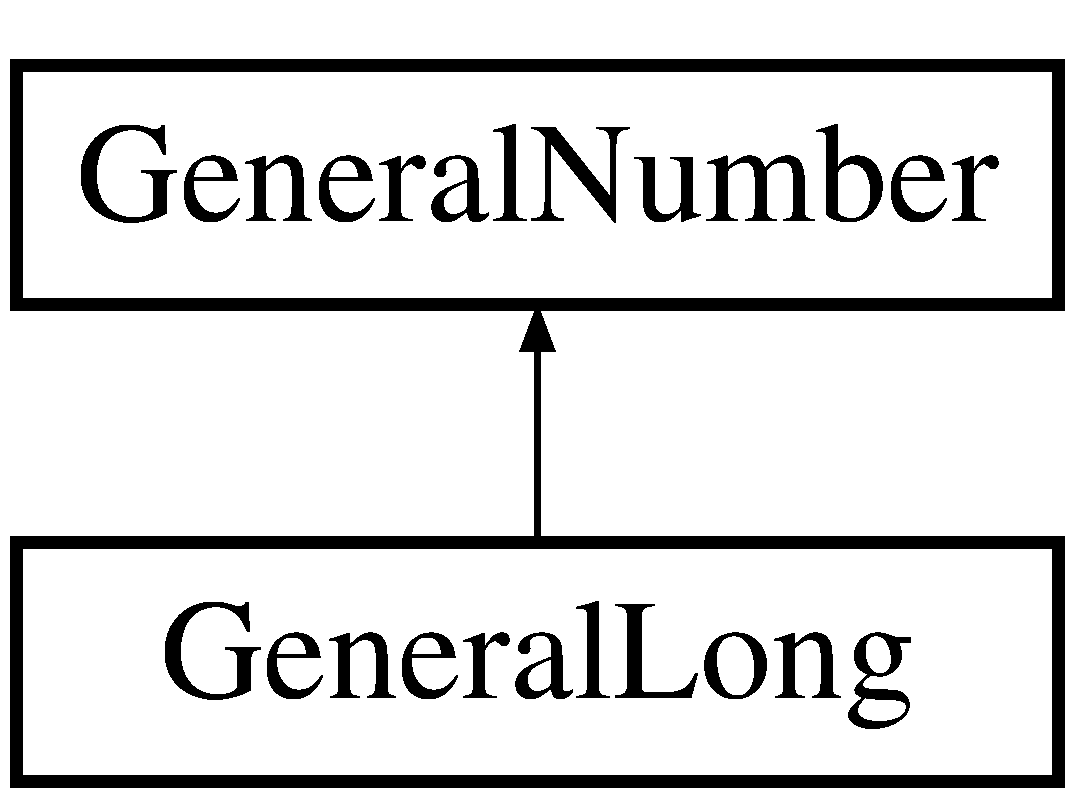
\includegraphics[height=2.000000cm]{classGeneralLong}
\end{center}
\end{figure}
\subsection*{Public Member Functions}
\begin{DoxyCompactItemize}
\item 
{\bf General\+Long} ()
\item 
{\bf General\+Long} (long {\bf value})
\item 
char $\ast$ {\bf to\+String} () const 
\item 
char $\ast$ {\bf foo} () const 
\item 
{\bf General\+Long} $\ast$ {\bf to\+General\+Long} () const 
\item 
{\bf General\+Rational} $\ast$ {\bf to\+General\+Rational} () const 
\item 
{\bf General\+Number} $\ast$ {\bf add} ({\bf General\+Number} $\ast$gn) const 
\end{DoxyCompactItemize}
\subsection*{Private Attributes}
\begin{DoxyCompactItemize}
\item 
long {\bf value}
\end{DoxyCompactItemize}


\subsection{Constructor \& Destructor Documentation}
\index{General\+Long@{General\+Long}!General\+Long@{General\+Long}}
\index{General\+Long@{General\+Long}!General\+Long@{General\+Long}}
\subsubsection[{General\+Long()}]{\setlength{\rightskip}{0pt plus 5cm}General\+Long\+::\+General\+Long (
\begin{DoxyParamCaption}
{}
\end{DoxyParamCaption}
)}\label{classGeneralLong_a9ba8d9844c5826284493301e3834e0fa}
Default constructor for \doxyref{General\+Long}{p.}{classGeneralLong} \index{General\+Long@{General\+Long}!General\+Long@{General\+Long}}
\index{General\+Long@{General\+Long}!General\+Long@{General\+Long}}
\subsubsection[{General\+Long(long value)}]{\setlength{\rightskip}{0pt plus 5cm}General\+Long\+::\+General\+Long (
\begin{DoxyParamCaption}
\item[{long}]{value}
\end{DoxyParamCaption}
)}\label{classGeneralLong_ac76419bcc51c55390d4b886f4c1ea828}
Constructor for \doxyref{General\+Long}{p.}{classGeneralLong} 
\begin{DoxyParams}{Parameters}
{\em value} & Number to store in the object \\
\hline
\end{DoxyParams}


\subsection{Member Function Documentation}
\index{General\+Long@{General\+Long}!add@{add}}
\index{add@{add}!General\+Long@{General\+Long}}
\subsubsection[{add(\+General\+Number $\ast$gn) const }]{\setlength{\rightskip}{0pt plus 5cm}{\bf General\+Number} $\ast$ General\+Long\+::add (
\begin{DoxyParamCaption}
\item[{{\bf General\+Number} $\ast$}]{gn}
\end{DoxyParamCaption}
) const\hspace{0.3cm}{\ttfamily [virtual]}}\label{classGeneralLong_adc191c69da156fddec21f6e3fa782fbf}
Converts any \doxyref{General\+Number}{p.}{classGeneralNumber} to \doxyref{General\+Long}{p.}{classGeneralLong} and then adds the value of the object it is invoked on to the value found in the object it converted Then returns generates a \doxyref{General\+Long}{p.}{classGeneralLong} of the sum 
\begin{DoxyParams}{Parameters}
{\em gn} & \doxyref{General\+Number}{p.}{classGeneralNumber} we want added to the \doxyref{General\+Long}{p.}{classGeneralLong} \\
\hline
\end{DoxyParams}
\begin{DoxyReturn}{Returns}
Pointer to the sum in \doxyref{General\+Long}{p.}{classGeneralLong} form 
\end{DoxyReturn}


Reimplemented from {\bf General\+Number} \doxyref{}{p.}{classGeneralNumber_a93c44b96a6a8a8df9bb6e3d73359d528}.



References General\+Number\+::to\+General\+Long(), and value.



Referenced by main().

\index{General\+Long@{General\+Long}!foo@{foo}}
\index{foo@{foo}!General\+Long@{General\+Long}}
\subsubsection[{foo() const }]{\setlength{\rightskip}{0pt plus 5cm}char $\ast$ General\+Long\+::foo (
\begin{DoxyParamCaption}
{}
\end{DoxyParamCaption}
) const}\label{classGeneralLong_a9c7e995eb89b06f3db51c0b5faaa272c}
Demonstrates a non-\/virtual function. \begin{DoxyReturn}{Returns}
Freshly-\/allocated C-\/stype string 
\end{DoxyReturn}


Referenced by main().

\index{General\+Long@{General\+Long}!to\+General\+Long@{to\+General\+Long}}
\index{to\+General\+Long@{to\+General\+Long}!General\+Long@{General\+Long}}
\subsubsection[{to\+General\+Long() const }]{\setlength{\rightskip}{0pt plus 5cm}{\bf General\+Long} $\ast$ General\+Long\+::to\+General\+Long (
\begin{DoxyParamCaption}
{}
\end{DoxyParamCaption}
) const\hspace{0.3cm}{\ttfamily [virtual]}}\label{classGeneralLong_a67fdd908d3af4a8fefc0657f2eb86dd0}
Generates an equivalent \doxyref{General\+Long}{p.}{classGeneralLong} \begin{DoxyReturn}{Returns}
Pointer to a freshly-\/allocated \doxyref{General\+Long}{p.}{classGeneralLong} object 
\end{DoxyReturn}


Reimplemented from {\bf General\+Number} \doxyref{}{p.}{classGeneralNumber_a3257176764dd42f884f3d32bc26cd508}.

\index{General\+Long@{General\+Long}!to\+General\+Rational@{to\+General\+Rational}}
\index{to\+General\+Rational@{to\+General\+Rational}!General\+Long@{General\+Long}}
\subsubsection[{to\+General\+Rational() const }]{\setlength{\rightskip}{0pt plus 5cm}{\bf General\+Rational} $\ast$ General\+Long\+::to\+General\+Rational (
\begin{DoxyParamCaption}
{}
\end{DoxyParamCaption}
) const\hspace{0.3cm}{\ttfamily [virtual]}}\label{classGeneralLong_aa983396c8843991c6bbea52b1d22e51b}
Generates an equivalent \doxyref{General\+Rational}{p.}{classGeneralRational} \begin{DoxyReturn}{Returns}
Pointer to a freshly-\/allocated \doxyref{General\+Rational}{p.}{classGeneralRational} object 
\end{DoxyReturn}


Reimplemented from {\bf General\+Number} \doxyref{}{p.}{classGeneralNumber_ae92a1bfb38c40bcda30fd93335a4ea54}.



Referenced by main().

\index{General\+Long@{General\+Long}!to\+String@{to\+String}}
\index{to\+String@{to\+String}!General\+Long@{General\+Long}}
\subsubsection[{to\+String() const }]{\setlength{\rightskip}{0pt plus 5cm}char $\ast$ General\+Long\+::to\+String (
\begin{DoxyParamCaption}
{}
\end{DoxyParamCaption}
) const\hspace{0.3cm}{\ttfamily [virtual]}}\label{classGeneralLong_ae3afbc099d82bf5a8eb7d8e9ac32cb87}
Generates a printable representation of the object. \begin{DoxyReturn}{Returns}
Freshly-\/allocated C-\/stype string 
\end{DoxyReturn}


Reimplemented from {\bf General\+Number} \doxyref{}{p.}{classGeneralNumber_a071819b67064dc17754ff7cdc4964d75}.



References M\+A\+X\+\_\+\+D\+I\+G\+I\+T\+S\+\_\+\+I\+N\+\_\+\+L\+O\+NG.



Referenced by main().



\subsection{Member Data Documentation}
\index{General\+Long@{General\+Long}!value@{value}}
\index{value@{value}!General\+Long@{General\+Long}}
\subsubsection[{value}]{\setlength{\rightskip}{0pt plus 5cm}long General\+Long\+::value\hspace{0.3cm}{\ttfamily [private]}}\label{classGeneralLong_a3a25ceb37f06367fd5cf2b22e97289aa}


Referenced by add().



The documentation for this class was generated from the following files\+:\begin{DoxyCompactItemize}
\item 
{\bf General\+Number.\+h}\item 
{\bf General\+Number.\+cpp}\end{DoxyCompactItemize}

\section{General\+Number Class Reference}
\label{classGeneralNumber}\index{General\+Number@{General\+Number}}


{\ttfamily \#include $<$General\+Number.\+h$>$}

Inheritance diagram for General\+Number\+:\begin{figure}[H]
\begin{center}
\leavevmode
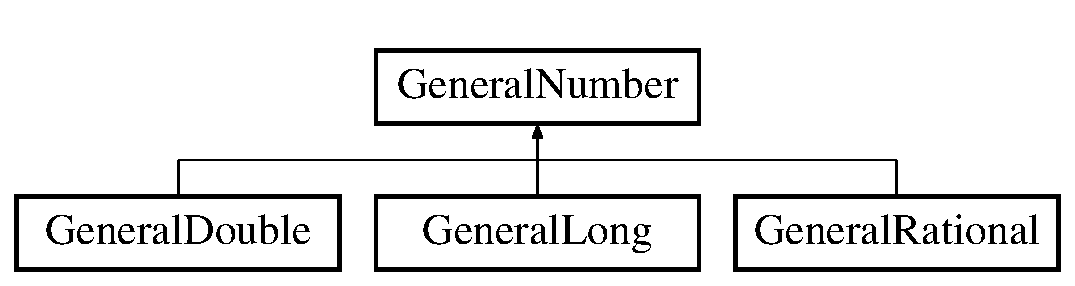
\includegraphics[height=2.000000cm]{classGeneralNumber}
\end{center}
\end{figure}
\subsection*{Public Member Functions}
\begin{DoxyCompactItemize}
\item 
{\bf General\+Number} ()
\item 
virtual char $\ast$ {\bf to\+String} () const 
\item 
char $\ast$ {\bf foo} () const 
\item 
virtual {\bf General\+Long} $\ast$ {\bf to\+General\+Long} () const 
\item 
virtual {\bf General\+Rational} $\ast$ {\bf to\+General\+Rational} () const 
\item 
virtual {\bf General\+Number} $\ast$ {\bf add} ({\bf General\+Number} $\ast$g) const 
\end{DoxyCompactItemize}


\subsection{Constructor \& Destructor Documentation}
\index{General\+Number@{General\+Number}!General\+Number@{General\+Number}}
\index{General\+Number@{General\+Number}!General\+Number@{General\+Number}}
\subsubsection[{General\+Number()}]{\setlength{\rightskip}{0pt plus 5cm}General\+Number\+::\+General\+Number (
\begin{DoxyParamCaption}
{}
\end{DoxyParamCaption}
)}\label{classGeneralNumber_a3c08bdccb4a03c82932546d5c19e636d}
Default constructor for \doxyref{General\+Number}{p.}{classGeneralNumber} 

\subsection{Member Function Documentation}
\index{General\+Number@{General\+Number}!add@{add}}
\index{add@{add}!General\+Number@{General\+Number}}
\subsubsection[{add(\+General\+Number $\ast$g) const }]{\setlength{\rightskip}{0pt plus 5cm}{\bf General\+Number} $\ast$ General\+Number\+::add (
\begin{DoxyParamCaption}
\item[{{\bf General\+Number} $\ast$}]{g}
\end{DoxyParamCaption}
) const\hspace{0.3cm}{\ttfamily [virtual]}}\label{classGeneralNumber_a93c44b96a6a8a8df9bb6e3d73359d528}
Returns pointer to \doxyref{General\+Number}{p.}{classGeneralNumber} \begin{DoxyReturn}{Returns}
Pointer to the \doxyref{General\+Number}{p.}{classGeneralNumber} passed in 
\end{DoxyReturn}


Reimplemented in {\bf General\+Rational} \doxyref{}{p.}{classGeneralRational_ad9e849aee88d19f5c7c272104b76ce70}, and {\bf General\+Long} \doxyref{}{p.}{classGeneralLong_adc191c69da156fddec21f6e3fa782fbf}.

\index{General\+Number@{General\+Number}!foo@{foo}}
\index{foo@{foo}!General\+Number@{General\+Number}}
\subsubsection[{foo() const }]{\setlength{\rightskip}{0pt plus 5cm}char $\ast$ General\+Number\+::foo (
\begin{DoxyParamCaption}
{}
\end{DoxyParamCaption}
) const}\label{classGeneralNumber_afedc95deda6c653dd57485930865b6ca}
Demonstrates a non-\/virtual function. \begin{DoxyReturn}{Returns}
Freshly-\/allocated C-\/stype string 
\end{DoxyReturn}


Referenced by main().

\index{General\+Number@{General\+Number}!to\+General\+Long@{to\+General\+Long}}
\index{to\+General\+Long@{to\+General\+Long}!General\+Number@{General\+Number}}
\subsubsection[{to\+General\+Long() const }]{\setlength{\rightskip}{0pt plus 5cm}{\bf General\+Long} $\ast$ General\+Number\+::to\+General\+Long (
\begin{DoxyParamCaption}
{}
\end{DoxyParamCaption}
) const\hspace{0.3cm}{\ttfamily [virtual]}}\label{classGeneralNumber_a3257176764dd42f884f3d32bc26cd508}
Generates an equivalent \doxyref{General\+Long}{p.}{classGeneralLong} \begin{DoxyReturn}{Returns}
Pointer to a freshly-\/allocated \doxyref{General\+Long}{p.}{classGeneralLong} object 
\end{DoxyReturn}


Reimplemented in {\bf General\+Rational} \doxyref{}{p.}{classGeneralRational_aadd587b17b9ce5bc6beea2bf065e68ca}, and {\bf General\+Long} \doxyref{}{p.}{classGeneralLong_a67fdd908d3af4a8fefc0657f2eb86dd0}.



Referenced by General\+Long\+::add(), and main().

\index{General\+Number@{General\+Number}!to\+General\+Rational@{to\+General\+Rational}}
\index{to\+General\+Rational@{to\+General\+Rational}!General\+Number@{General\+Number}}
\subsubsection[{to\+General\+Rational() const }]{\setlength{\rightskip}{0pt plus 5cm}{\bf General\+Rational} $\ast$ General\+Number\+::to\+General\+Rational (
\begin{DoxyParamCaption}
{}
\end{DoxyParamCaption}
) const\hspace{0.3cm}{\ttfamily [virtual]}}\label{classGeneralNumber_ae92a1bfb38c40bcda30fd93335a4ea54}
Generates an equivalent \doxyref{General\+Rational}{p.}{classGeneralRational} \begin{DoxyReturn}{Returns}
Pointer to a freshly-\/allocated \doxyref{General\+Rational}{p.}{classGeneralRational} object 
\end{DoxyReturn}


Reimplemented in {\bf General\+Rational} \doxyref{}{p.}{classGeneralRational_af474c9b5f3f31934c24ba47230cd5537}, and {\bf General\+Long} \doxyref{}{p.}{classGeneralLong_aa983396c8843991c6bbea52b1d22e51b}.



Referenced by General\+Rational\+::add().

\index{General\+Number@{General\+Number}!to\+String@{to\+String}}
\index{to\+String@{to\+String}!General\+Number@{General\+Number}}
\subsubsection[{to\+String() const }]{\setlength{\rightskip}{0pt plus 5cm}char $\ast$ General\+Number\+::to\+String (
\begin{DoxyParamCaption}
{}
\end{DoxyParamCaption}
) const\hspace{0.3cm}{\ttfamily [virtual]}}\label{classGeneralNumber_a071819b67064dc17754ff7cdc4964d75}
Generates a printable representation of the object. \begin{DoxyReturn}{Returns}
Freshly-\/allocated C-\/stype string 
\end{DoxyReturn}


Reimplemented in {\bf General\+Rational} \doxyref{}{p.}{classGeneralRational_a592adc36a0593c960c197741ab5b50b9}, and {\bf General\+Long} \doxyref{}{p.}{classGeneralLong_ae3afbc099d82bf5a8eb7d8e9ac32cb87}.



Referenced by main().



The documentation for this class was generated from the following files\+:\begin{DoxyCompactItemize}
\item 
{\bf General\+Number.\+h}\item 
{\bf General\+Number.\+cpp}\end{DoxyCompactItemize}

\section{General\+Rational Class Reference}
\label{classGeneralRational}\index{General\+Rational@{General\+Rational}}


{\ttfamily \#include $<$General\+Number.\+h$>$}

Inheritance diagram for General\+Rational\+:\begin{figure}[H]
\begin{center}
\leavevmode
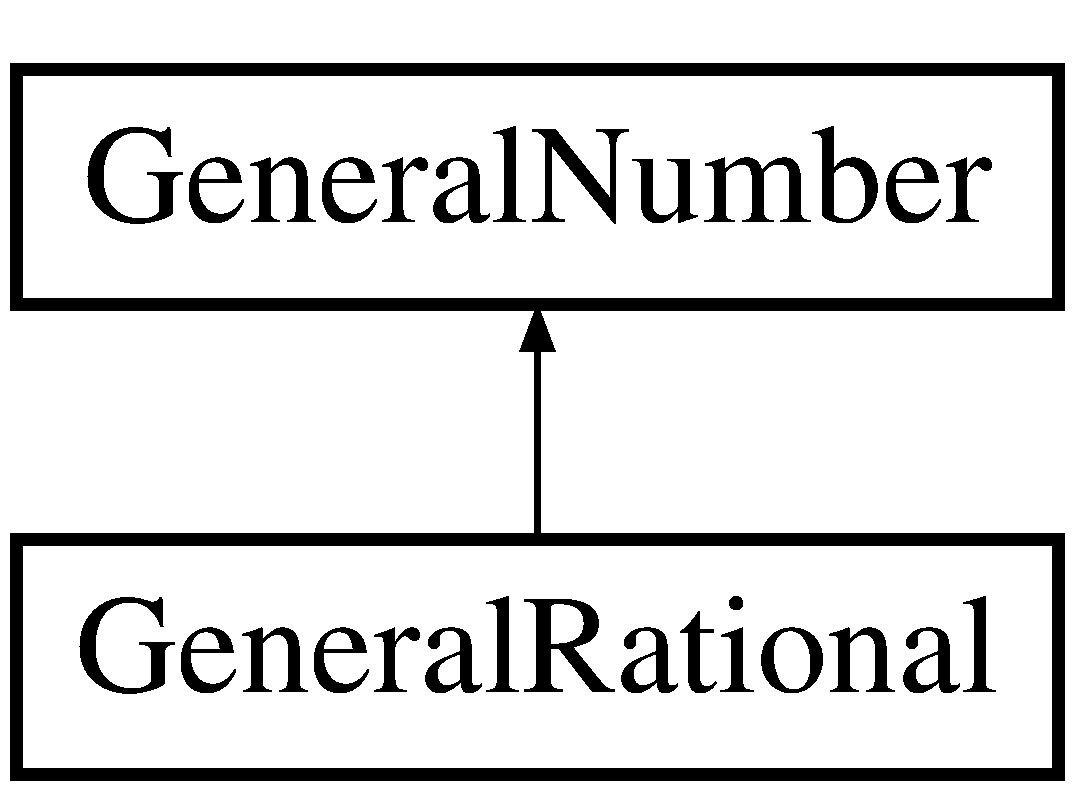
\includegraphics[height=2.000000cm]{classGeneralRational}
\end{center}
\end{figure}
\subsection*{Public Member Functions}
\begin{DoxyCompactItemize}
\item 
{\bf General\+Rational} ()
\item 
{\bf General\+Rational} (long {\bf top}, long {\bf bottom})
\item 
char $\ast$ {\bf to\+String} () const 
\item 
char $\ast$ {\bf foo} () const 
\item 
{\bf General\+Long} $\ast$ {\bf to\+General\+Long} () const 
\item 
{\bf General\+Rational} $\ast$ {\bf to\+General\+Rational} () const 
\item 
{\bf General\+Double} $\ast$ {\bf to\+General\+Double} () const 
\item 
void {\bf to\+Canonical\+Form} ()
\item 
{\bf General\+Number} $\ast$ {\bf add} ({\bf General\+Number} $\ast$gn) const 
\item 
{\bf General\+Number} $\ast$ {\bf subtract} ({\bf General\+Number} $\ast$gn) const 
\item 
{\bf General\+Number} $\ast$ {\bf multiply} ({\bf General\+Number} $\ast$gn) const 
\item 
{\bf General\+Number} $\ast$ {\bf divide} ({\bf General\+Number} $\ast$gn) const 
\end{DoxyCompactItemize}
\subsection*{Private Attributes}
\begin{DoxyCompactItemize}
\item 
long {\bf top}
\item 
long {\bf bottom}
\end{DoxyCompactItemize}
\subsection*{Additional Inherited Members}


\subsection{Constructor \& Destructor Documentation}
\index{General\+Rational@{General\+Rational}!General\+Rational@{General\+Rational}}
\index{General\+Rational@{General\+Rational}!General\+Rational@{General\+Rational}}
\subsubsection[{General\+Rational()}]{\setlength{\rightskip}{0pt plus 5cm}General\+Rational\+::\+General\+Rational (
\begin{DoxyParamCaption}
{}
\end{DoxyParamCaption}
)}\label{classGeneralRational_a681f589c9e7699dbb1fdafd136abf325}
Default constructor for \doxyref{General\+Rational}{p.}{classGeneralRational} \index{General\+Rational@{General\+Rational}!General\+Rational@{General\+Rational}}
\index{General\+Rational@{General\+Rational}!General\+Rational@{General\+Rational}}
\subsubsection[{General\+Rational(long top, long bottom)}]{\setlength{\rightskip}{0pt plus 5cm}General\+Rational\+::\+General\+Rational (
\begin{DoxyParamCaption}
\item[{long}]{top, }
\item[{long}]{bottom}
\end{DoxyParamCaption}
)}\label{classGeneralRational_aa6f7a00036226fa620d77ac1a345fae0}
Constructor for \doxyref{General\+Rational}{p.}{classGeneralRational} 
\begin{DoxyParams}{Parameters}
{\em top} & Numerator to store in the object \\
\hline
{\em bottom} & Denominator to store in the object \\
\hline
\end{DoxyParams}


\subsection{Member Function Documentation}
\index{General\+Rational@{General\+Rational}!add@{add}}
\index{add@{add}!General\+Rational@{General\+Rational}}
\subsubsection[{add(\+General\+Number $\ast$gn) const }]{\setlength{\rightskip}{0pt plus 5cm}{\bf General\+Number} $\ast$ General\+Rational\+::add (
\begin{DoxyParamCaption}
\item[{{\bf General\+Number} $\ast$}]{gn}
\end{DoxyParamCaption}
) const\hspace{0.3cm}{\ttfamily [virtual]}}\label{classGeneralRational_ad9e849aee88d19f5c7c272104b76ce70}
Converts \doxyref{General\+Number}{p.}{classGeneralNumber} passed in to \doxyref{General\+Rational}{p.}{classGeneralRational} and adds its value with the converted General\+Ration by the help of lcm() helper function. 
\begin{DoxyParams}{Parameters}
{\em gn} & \doxyref{General\+Number}{p.}{classGeneralNumber} we wanted added to the \doxyref{General\+Rational}{p.}{classGeneralRational} \\
\hline
\end{DoxyParams}
\begin{DoxyReturn}{Returns}
Pointer to the sum in \doxyref{General\+Rational}{p.}{classGeneralRational} form 
\end{DoxyReturn}


Implements {\bf General\+Number} \doxyref{}{p.}{classGeneralNumber_abf66663792afad01a954d0326ee28bc7}.



References bottom, find\+\_\+lcd(), to\+Canonical\+Form(), General\+Number\+::to\+General\+Rational(), and top.



Referenced by main().

\index{General\+Rational@{General\+Rational}!divide@{divide}}
\index{divide@{divide}!General\+Rational@{General\+Rational}}
\subsubsection[{divide(\+General\+Number $\ast$gn) const }]{\setlength{\rightskip}{0pt plus 5cm}{\bf General\+Number} $\ast$ General\+Rational\+::divide (
\begin{DoxyParamCaption}
\item[{{\bf General\+Number} $\ast$}]{gn}
\end{DoxyParamCaption}
) const\hspace{0.3cm}{\ttfamily [virtual]}}\label{classGeneralRational_a81b9d20f4ce3b2109ee6eeee9334aedd}
Converts \doxyref{General\+Number}{p.}{classGeneralNumber} passed in to \doxyref{General\+Rational}{p.}{classGeneralRational} and divides its value with the converted \doxyref{General\+Rational}{p.}{classGeneralRational} by inverting the top and bottom values of the converted value and multiplying the object with it. Then returns the result in \doxyref{General\+Rational}{p.}{classGeneralRational} form. 
\begin{DoxyParams}{Parameters}
{\em gn} & \doxyref{General\+Number}{p.}{classGeneralNumber} we wanted to divide the \doxyref{General\+Rational}{p.}{classGeneralRational} with \\
\hline
\end{DoxyParams}
\begin{DoxyReturn}{Returns}
Pointer to the quotient in \doxyref{General\+Rational}{p.}{classGeneralRational} form 
\end{DoxyReturn}


Implements {\bf General\+Number} \doxyref{}{p.}{classGeneralNumber_a00210335039ff12f5d8cc8d94949a031}.



References bottom, to\+Canonical\+Form(), General\+Number\+::to\+General\+Rational(), and top.

\index{General\+Rational@{General\+Rational}!foo@{foo}}
\index{foo@{foo}!General\+Rational@{General\+Rational}}
\subsubsection[{foo() const }]{\setlength{\rightskip}{0pt plus 5cm}char $\ast$ General\+Rational\+::foo (
\begin{DoxyParamCaption}
{}
\end{DoxyParamCaption}
) const}\label{classGeneralRational_a265451cfed295bc3711cf532ffa28d03}
Demonstrates a non-\/virtual function. \begin{DoxyReturn}{Returns}
Freshly-\/allocated C-\/stype string 
\end{DoxyReturn}
\index{General\+Rational@{General\+Rational}!multiply@{multiply}}
\index{multiply@{multiply}!General\+Rational@{General\+Rational}}
\subsubsection[{multiply(\+General\+Number $\ast$gn) const }]{\setlength{\rightskip}{0pt plus 5cm}{\bf General\+Number} $\ast$ General\+Rational\+::multiply (
\begin{DoxyParamCaption}
\item[{{\bf General\+Number} $\ast$}]{gn}
\end{DoxyParamCaption}
) const\hspace{0.3cm}{\ttfamily [virtual]}}\label{classGeneralRational_a52f58fb3f7f1e21f5399e88d646182b5}
Converts \doxyref{General\+Number}{p.}{classGeneralNumber} passed in to \doxyref{General\+Rational}{p.}{classGeneralRational} and multiplies its top and bottom values with the converted \doxyref{General\+Rational}{p.}{classGeneralRational}\textquotesingle{}s top and bottom values and then return\textquotesingle{}s the result in \doxyref{General\+Rational}{p.}{classGeneralRational} form. 
\begin{DoxyParams}{Parameters}
{\em gn} & \doxyref{General\+Number}{p.}{classGeneralNumber} we wanted multiplied to the \doxyref{General\+Rational}{p.}{classGeneralRational} \\
\hline
\end{DoxyParams}
\begin{DoxyReturn}{Returns}
Pointer to the sum in \doxyref{General\+Rational}{p.}{classGeneralRational} form 
\end{DoxyReturn}


Implements {\bf General\+Number} \doxyref{}{p.}{classGeneralNumber_ac47d6c7deb64e3eee073a1e5105045fb}.



References bottom, to\+Canonical\+Form(), General\+Number\+::to\+General\+Rational(), and top.

\index{General\+Rational@{General\+Rational}!subtract@{subtract}}
\index{subtract@{subtract}!General\+Rational@{General\+Rational}}
\subsubsection[{subtract(\+General\+Number $\ast$gn) const }]{\setlength{\rightskip}{0pt plus 5cm}{\bf General\+Number} $\ast$ General\+Rational\+::subtract (
\begin{DoxyParamCaption}
\item[{{\bf General\+Number} $\ast$}]{gn}
\end{DoxyParamCaption}
) const\hspace{0.3cm}{\ttfamily [virtual]}}\label{classGeneralRational_a7b591901f7dfe12920d7fd3088bb97ff}
Converts \doxyref{General\+Number}{p.}{classGeneralNumber} passed in to \doxyref{General\+Rational}{p.}{classGeneralRational} and subtracts its value with the converted \doxyref{General\+Rational}{p.}{classGeneralRational} by the help of lcm() helper function. 
\begin{DoxyParams}{Parameters}
{\em gn} & \doxyref{General\+Number}{p.}{classGeneralNumber} we wanted subtracted from the \doxyref{General\+Rational}{p.}{classGeneralRational} \\
\hline
\end{DoxyParams}
\begin{DoxyReturn}{Returns}
Pointer to the sum in \doxyref{General\+Rational}{p.}{classGeneralRational} form 
\end{DoxyReturn}


Implements {\bf General\+Number} \doxyref{}{p.}{classGeneralNumber_ae9010718fcbc6fcfe54faabdd19408de}.



References bottom, find\+\_\+lcd(), to\+Canonical\+Form(), General\+Number\+::to\+General\+Rational(), and top.

\index{General\+Rational@{General\+Rational}!to\+Canonical\+Form@{to\+Canonical\+Form}}
\index{to\+Canonical\+Form@{to\+Canonical\+Form}!General\+Rational@{General\+Rational}}
\subsubsection[{to\+Canonical\+Form()}]{\setlength{\rightskip}{0pt plus 5cm}void General\+Rational\+::to\+Canonical\+Form (
\begin{DoxyParamCaption}
{}
\end{DoxyParamCaption}
)}\label{classGeneralRational_a40a30e4d4386054abf0ceeacbebd6b1a}
Finds the G\+CD of the nominator and denominator and divides them with their G\+CD to fing their lowest term. Also arranges position of negative sign \begin{DoxyReturn}{Returns}
Same \doxyref{General\+Rational}{p.}{classGeneralRational} but in lowest term/canonical form 
\end{DoxyReturn}


References find\+\_\+gcd(), and gcd().



Referenced by add(), divide(), main(), multiply(), and subtract().

\index{General\+Rational@{General\+Rational}!to\+General\+Double@{to\+General\+Double}}
\index{to\+General\+Double@{to\+General\+Double}!General\+Rational@{General\+Rational}}
\subsubsection[{to\+General\+Double() const }]{\setlength{\rightskip}{0pt plus 5cm}{\bf General\+Double} $\ast$ General\+Rational\+::to\+General\+Double (
\begin{DoxyParamCaption}
{}
\end{DoxyParamCaption}
) const\hspace{0.3cm}{\ttfamily [virtual]}}\label{classGeneralRational_a45714e227a97f7dafdcff19ed87e2cbd}
Generates an equivalent \doxyref{General\+Double}{p.}{classGeneralDouble} \begin{DoxyReturn}{Returns}
Pointer to a freshly-\/allocated \doxyref{General\+Double}{p.}{classGeneralDouble} object 
\end{DoxyReturn}


Implements {\bf General\+Number} \doxyref{}{p.}{classGeneralNumber_a597b8ff270d49970f70b0ba6e5246593}.

\index{General\+Rational@{General\+Rational}!to\+General\+Long@{to\+General\+Long}}
\index{to\+General\+Long@{to\+General\+Long}!General\+Rational@{General\+Rational}}
\subsubsection[{to\+General\+Long() const }]{\setlength{\rightskip}{0pt plus 5cm}{\bf General\+Long} $\ast$ General\+Rational\+::to\+General\+Long (
\begin{DoxyParamCaption}
{}
\end{DoxyParamCaption}
) const\hspace{0.3cm}{\ttfamily [virtual]}}\label{classGeneralRational_aadd587b17b9ce5bc6beea2bf065e68ca}
Generates an equivalent \doxyref{General\+Long}{p.}{classGeneralLong} \begin{DoxyReturn}{Returns}
Pointer to a freshly-\/allocated \doxyref{General\+Long}{p.}{classGeneralLong} object 
\end{DoxyReturn}


Implements {\bf General\+Number} \doxyref{}{p.}{classGeneralNumber_acafc7321465d601588e47dc270bf147a}.



Referenced by main().

\index{General\+Rational@{General\+Rational}!to\+General\+Rational@{to\+General\+Rational}}
\index{to\+General\+Rational@{to\+General\+Rational}!General\+Rational@{General\+Rational}}
\subsubsection[{to\+General\+Rational() const }]{\setlength{\rightskip}{0pt plus 5cm}{\bf General\+Rational} $\ast$ General\+Rational\+::to\+General\+Rational (
\begin{DoxyParamCaption}
{}
\end{DoxyParamCaption}
) const\hspace{0.3cm}{\ttfamily [virtual]}}\label{classGeneralRational_af474c9b5f3f31934c24ba47230cd5537}
Generates an equivalent \doxyref{General\+Rational}{p.}{classGeneralRational} \begin{DoxyReturn}{Returns}
Pointer to a freshly-\/allocated \doxyref{General\+Rational}{p.}{classGeneralRational} object 
\end{DoxyReturn}


Implements {\bf General\+Number} \doxyref{}{p.}{classGeneralNumber_aec6e631e5b839b50224f5c2b76eb1162}.

\index{General\+Rational@{General\+Rational}!to\+String@{to\+String}}
\index{to\+String@{to\+String}!General\+Rational@{General\+Rational}}
\subsubsection[{to\+String() const }]{\setlength{\rightskip}{0pt plus 5cm}char $\ast$ General\+Rational\+::to\+String (
\begin{DoxyParamCaption}
{}
\end{DoxyParamCaption}
) const\hspace{0.3cm}{\ttfamily [virtual]}}\label{classGeneralRational_a592adc36a0593c960c197741ab5b50b9}
Generates a printable representation of the object. \begin{DoxyReturn}{Returns}
Freshly-\/allocated C-\/stype string 
\end{DoxyReturn}


Implements {\bf General\+Number} \doxyref{}{p.}{classGeneralNumber_aa3a0cdda717ff1e29d7c0c6ab2684b70}.



References M\+A\+X\+\_\+\+D\+I\+G\+I\+T\+S\+\_\+\+I\+N\+\_\+\+L\+O\+NG.



Referenced by main().



\subsection{Member Data Documentation}
\index{General\+Rational@{General\+Rational}!bottom@{bottom}}
\index{bottom@{bottom}!General\+Rational@{General\+Rational}}
\subsubsection[{bottom}]{\setlength{\rightskip}{0pt plus 5cm}long General\+Rational\+::bottom\hspace{0.3cm}{\ttfamily [private]}}\label{classGeneralRational_a74835ffcc9a7b1026658da2fb75dc0d7}


Referenced by add(), divide(), multiply(), and subtract().

\index{General\+Rational@{General\+Rational}!top@{top}}
\index{top@{top}!General\+Rational@{General\+Rational}}
\subsubsection[{top}]{\setlength{\rightskip}{0pt plus 5cm}long General\+Rational\+::top\hspace{0.3cm}{\ttfamily [private]}}\label{classGeneralRational_a771617023f9c874e6920b001ab394a57}


Referenced by add(), divide(), multiply(), and subtract().



The documentation for this class was generated from the following files\+:\begin{DoxyCompactItemize}
\item 
{\bf General\+Number.\+h}\item 
{\bf General\+Number.\+cpp}\end{DoxyCompactItemize}

\chapter{File Documentation}
\section{calc.\+cpp File Reference}
\label{calc_8cpp}\index{calc.\+cpp@{calc.\+cpp}}
{\ttfamily \#include $<$iostream$>$}\\*
{\ttfamily \#include $<$stdio.\+h$>$}\\*
{\ttfamily \#include $<$stdlib.\+h$>$}\\*
{\ttfamily \#include $<$string.\+h$>$}\\*
{\ttfamily \#include \char`\"{}General\+Number.\+h\char`\"{}}\\*
\subsection*{Functions}
\begin{DoxyCompactItemize}
\item 
int {\bf main} (int argc, char $\ast$argv[$\,$])
\item 
int {\bf start\+\_\+calculator} ()
\item 
{\bf General\+Number} $\ast$ {\bf calculate} ({\bf General\+Number} $\ast$fnum, {\bf General\+Number} $\ast$snum, char $\ast$oprtr)
\end{DoxyCompactItemize}


\subsection{Function Documentation}
\index{calc.\+cpp@{calc.\+cpp}!calculate@{calculate}}
\index{calculate@{calculate}!calc.\+cpp@{calc.\+cpp}}
\subsubsection[{calculate(\+General\+Number $\ast$fnum, General\+Number $\ast$snum, char $\ast$oprtr)}]{\setlength{\rightskip}{0pt plus 5cm}{\bf General\+Number}$\ast$ calculate (
\begin{DoxyParamCaption}
\item[{{\bf General\+Number} $\ast$}]{fnum, }
\item[{{\bf General\+Number} $\ast$}]{snum, }
\item[{char $\ast$}]{oprtr}
\end{DoxyParamCaption}
)}\label{calc_8cpp_a75b8be442566a5970c667ec91805fbe5}
Consumes two General\+Numbers and an operation (string form) and then and then uses helper functions to apply operations on the given objects and then9 return the answer in \doxyref{General\+Number}{p.}{classGeneralNumber} object form 
\begin{DoxyParams}{Parameters}
{\em fnum} & Number the second number will be applied on by the operation \\
\hline
{\em snum} & Number that will be applied on the first number by the operation \\
\hline
{\em oprtr} & Operator to be applied in string form \\
\hline
\end{DoxyParams}
\begin{DoxyReturn}{Returns}
Answer of the operation on the two numbers in \doxyref{General\+Number}{p.}{classGeneralNumber} form 
\end{DoxyReturn}


References General\+Number\+::add(), General\+Number\+::divide(), General\+Number\+::multiply(), and General\+Number\+::subtract().



Referenced by start\+\_\+calculator().

\index{calc.\+cpp@{calc.\+cpp}!main@{main}}
\index{main@{main}!calc.\+cpp@{calc.\+cpp}}
\subsubsection[{main(int argc, char $\ast$argv[])}]{\setlength{\rightskip}{0pt plus 5cm}int main (
\begin{DoxyParamCaption}
\item[{int}]{argc, }
\item[{char $\ast$}]{argv[$\,$]}
\end{DoxyParamCaption}
)}\label{calc_8cpp_a0ddf1224851353fc92bfbff6f499fa97}
Calculator program using \doxyref{General\+Number}{p.}{classGeneralNumber} class and its subclasses. 
\begin{DoxyParams}{Parameters}
{\em argc} & Number of words on the command line. \\
\hline
{\em argv} & Array of pointers to these words. \\
\hline
\end{DoxyParams}


References start\+\_\+calculator().

\index{calc.\+cpp@{calc.\+cpp}!start\+\_\+calculator@{start\+\_\+calculator}}
\index{start\+\_\+calculator@{start\+\_\+calculator}!calc.\+cpp@{calc.\+cpp}}
\subsubsection[{start\+\_\+calculator()}]{\setlength{\rightskip}{0pt plus 5cm}int start\+\_\+calculator (
\begin{DoxyParamCaption}
{}
\end{DoxyParamCaption}
)}\label{calc_8cpp_a3ec86ab3ebbc502171aec4af40b1c6d3}
Asks user to enter two numbers (arguments in string form) and an operation (char) and then parses those number to \doxyref{General\+Number}{p.}{classGeneralNumber} form and then calculates the result in accordance with the operation given \begin{DoxyReturn}{Returns}
0 or 1 to indicate when users want to end calculator (loop) 
\end{DoxyReturn}


References calculate(), M\+A\+X\+\_\+\+D\+I\+G\+I\+T\+S\+\_\+\+O\+R\+\_\+\+C\+H\+A\+R\+A\+C\+T\+E\+R\+S\+\_\+\+E\+N\+T\+E\+R\+ED, General\+Number\+::parse(), and General\+Number\+::to\+String().



Referenced by main().


\section{General\+Number.\+cpp File Reference}
\label{GeneralNumber_8cpp}\index{General\+Number.\+cpp@{General\+Number.\+cpp}}
{\ttfamily \#include $<$stdio.\+h$>$}\\*
{\ttfamily \#include $<$string.\+h$>$}\\*
{\ttfamily \#include $<$stdlib.\+h$>$}\\*
{\ttfamily \#include \char`\"{}General\+Number.\+h\char`\"{}}\\*
\subsection*{Functions}
\begin{DoxyCompactItemize}
\item 
long {\bf find\+\_\+gcd} (long a, long b)
\item 
long {\bf find\+\_\+lcd} (long a, long b)
\end{DoxyCompactItemize}


\subsection{Function Documentation}
\index{General\+Number.\+cpp@{General\+Number.\+cpp}!find\+\_\+gcd@{find\+\_\+gcd}}
\index{find\+\_\+gcd@{find\+\_\+gcd}!General\+Number.\+cpp@{General\+Number.\+cpp}}
\subsubsection[{find\+\_\+gcd(long a, long b)}]{\setlength{\rightskip}{0pt plus 5cm}long find\+\_\+gcd (
\begin{DoxyParamCaption}
\item[{long}]{a, }
\item[{long}]{b}
\end{DoxyParamCaption}
)}\label{GeneralNumber_8cpp_a3b1a81b44872a0bc193738b3762e1ec1}
Finds the Greatest Common Divisor of two numbers 
\begin{DoxyParams}{Parameters}
{\em a} & One of two numbers we want the G\+CD of \\
\hline
{\em b} & One of two numbers we want the G\+CD of \\
\hline
\end{DoxyParams}
\begin{DoxyReturn}{Returns}
The G\+CD of the two numbers in long format 
\end{DoxyReturn}


Referenced by find\+\_\+lcd(), and General\+Rational\+::to\+Canonical\+Form().

\index{General\+Number.\+cpp@{General\+Number.\+cpp}!find\+\_\+lcd@{find\+\_\+lcd}}
\index{find\+\_\+lcd@{find\+\_\+lcd}!General\+Number.\+cpp@{General\+Number.\+cpp}}
\subsubsection[{find\+\_\+lcd(long a, long b)}]{\setlength{\rightskip}{0pt plus 5cm}long find\+\_\+lcd (
\begin{DoxyParamCaption}
\item[{long}]{a, }
\item[{long}]{b}
\end{DoxyParamCaption}
)}\label{GeneralNumber_8cpp_a1a7f5010aff855526092e34b38b97bea}
Finds the Least Common Denominator of two numbers 
\begin{DoxyParams}{Parameters}
{\em a} & One of two numbers we want L\+CD of \\
\hline
{\em b} & One of two numbers we want L\+CD of \\
\hline
\end{DoxyParams}
\begin{DoxyReturn}{Returns}
The G\+CD of the two numbers in long format 
\end{DoxyReturn}


References find\+\_\+gcd().



Referenced by General\+Rational\+::add(), and General\+Rational\+::subtract().


\section{General\+Number.\+h File Reference}
\label{GeneralNumber_8h}\index{General\+Number.\+h@{General\+Number.\+h}}
\subsection*{Classes}
\begin{DoxyCompactItemize}
\item 
class {\bf General\+Number}
\item 
class {\bf General\+Long}
\item 
class {\bf General\+Rational}
\item 
class {\bf General\+Double}
\end{DoxyCompactItemize}
\subsection*{Macros}
\begin{DoxyCompactItemize}
\item 
\#define {\bf M\+A\+X\+\_\+\+D\+I\+G\+I\+T\+S\+\_\+\+I\+N\+\_\+\+L\+O\+NG}~(20)
\item 
\#define {\bf M\+A\+X\+\_\+\+D\+I\+G\+I\+T\+S\+\_\+\+I\+N\+\_\+\+D\+O\+U\+B\+LE}~(20)
\item 
\#define {\bf M\+A\+X\+\_\+\+D\+I\+G\+I\+T\+S\+\_\+\+O\+R\+\_\+\+C\+H\+A\+R\+A\+C\+T\+E\+R\+S\+\_\+\+E\+N\+T\+E\+R\+ED}~(20)
\end{DoxyCompactItemize}
\subsection*{Functions}
\begin{DoxyCompactItemize}
\item 
long {\bf find\+\_\+gcd} (long a, long b)
\item 
long {\bf find\+\_\+lcd} (long a, long b)
\item 
int {\bf start\+\_\+calculator} ()
\item 
{\bf General\+Number} $\ast$ {\bf calculate} ({\bf General\+Number} $\ast$fnum, {\bf General\+Number} $\ast$snum, char $\ast$oprtr)
\end{DoxyCompactItemize}


\subsection{Macro Definition Documentation}
\index{General\+Number.\+h@{General\+Number.\+h}!M\+A\+X\+\_\+\+D\+I\+G\+I\+T\+S\+\_\+\+I\+N\+\_\+\+D\+O\+U\+B\+LE@{M\+A\+X\+\_\+\+D\+I\+G\+I\+T\+S\+\_\+\+I\+N\+\_\+\+D\+O\+U\+B\+LE}}
\index{M\+A\+X\+\_\+\+D\+I\+G\+I\+T\+S\+\_\+\+I\+N\+\_\+\+D\+O\+U\+B\+LE@{M\+A\+X\+\_\+\+D\+I\+G\+I\+T\+S\+\_\+\+I\+N\+\_\+\+D\+O\+U\+B\+LE}!General\+Number.\+h@{General\+Number.\+h}}
\subsubsection[{M\+A\+X\+\_\+\+D\+I\+G\+I\+T\+S\+\_\+\+I\+N\+\_\+\+D\+O\+U\+B\+LE}]{\setlength{\rightskip}{0pt plus 5cm}\#define M\+A\+X\+\_\+\+D\+I\+G\+I\+T\+S\+\_\+\+I\+N\+\_\+\+D\+O\+U\+B\+LE~(20)}\label{GeneralNumber_8h_a6757e9c78c7325140af80150e4680a2c}


Referenced by General\+Double\+::to\+String().

\index{General\+Number.\+h@{General\+Number.\+h}!M\+A\+X\+\_\+\+D\+I\+G\+I\+T\+S\+\_\+\+I\+N\+\_\+\+L\+O\+NG@{M\+A\+X\+\_\+\+D\+I\+G\+I\+T\+S\+\_\+\+I\+N\+\_\+\+L\+O\+NG}}
\index{M\+A\+X\+\_\+\+D\+I\+G\+I\+T\+S\+\_\+\+I\+N\+\_\+\+L\+O\+NG@{M\+A\+X\+\_\+\+D\+I\+G\+I\+T\+S\+\_\+\+I\+N\+\_\+\+L\+O\+NG}!General\+Number.\+h@{General\+Number.\+h}}
\subsubsection[{M\+A\+X\+\_\+\+D\+I\+G\+I\+T\+S\+\_\+\+I\+N\+\_\+\+L\+O\+NG}]{\setlength{\rightskip}{0pt plus 5cm}\#define M\+A\+X\+\_\+\+D\+I\+G\+I\+T\+S\+\_\+\+I\+N\+\_\+\+L\+O\+NG~(20)}\label{GeneralNumber_8h_a4536bcf3e78506090145549baf064f59}


Referenced by General\+Long\+::to\+String(), and General\+Rational\+::to\+String().

\index{General\+Number.\+h@{General\+Number.\+h}!M\+A\+X\+\_\+\+D\+I\+G\+I\+T\+S\+\_\+\+O\+R\+\_\+\+C\+H\+A\+R\+A\+C\+T\+E\+R\+S\+\_\+\+E\+N\+T\+E\+R\+ED@{M\+A\+X\+\_\+\+D\+I\+G\+I\+T\+S\+\_\+\+O\+R\+\_\+\+C\+H\+A\+R\+A\+C\+T\+E\+R\+S\+\_\+\+E\+N\+T\+E\+R\+ED}}
\index{M\+A\+X\+\_\+\+D\+I\+G\+I\+T\+S\+\_\+\+O\+R\+\_\+\+C\+H\+A\+R\+A\+C\+T\+E\+R\+S\+\_\+\+E\+N\+T\+E\+R\+ED@{M\+A\+X\+\_\+\+D\+I\+G\+I\+T\+S\+\_\+\+O\+R\+\_\+\+C\+H\+A\+R\+A\+C\+T\+E\+R\+S\+\_\+\+E\+N\+T\+E\+R\+ED}!General\+Number.\+h@{General\+Number.\+h}}
\subsubsection[{M\+A\+X\+\_\+\+D\+I\+G\+I\+T\+S\+\_\+\+O\+R\+\_\+\+C\+H\+A\+R\+A\+C\+T\+E\+R\+S\+\_\+\+E\+N\+T\+E\+R\+ED}]{\setlength{\rightskip}{0pt plus 5cm}\#define M\+A\+X\+\_\+\+D\+I\+G\+I\+T\+S\+\_\+\+O\+R\+\_\+\+C\+H\+A\+R\+A\+C\+T\+E\+R\+S\+\_\+\+E\+N\+T\+E\+R\+ED~(20)}\label{GeneralNumber_8h_a561ca5dea9562e6e36b16c404a510a14}


Referenced by start\+\_\+calculator().



\subsection{Function Documentation}
\index{General\+Number.\+h@{General\+Number.\+h}!calculate@{calculate}}
\index{calculate@{calculate}!General\+Number.\+h@{General\+Number.\+h}}
\subsubsection[{calculate(\+General\+Number $\ast$fnum, General\+Number $\ast$snum, char $\ast$oprtr)}]{\setlength{\rightskip}{0pt plus 5cm}{\bf General\+Number}$\ast$ calculate (
\begin{DoxyParamCaption}
\item[{{\bf General\+Number} $\ast$}]{fnum, }
\item[{{\bf General\+Number} $\ast$}]{snum, }
\item[{char $\ast$}]{oprtr}
\end{DoxyParamCaption}
)}\label{GeneralNumber_8h_a75b8be442566a5970c667ec91805fbe5}
Consumes two General\+Numbers and an operation (string form) and then and then uses helper functions to apply operations on the given objects and then9 return the answer in \doxyref{General\+Number}{p.}{classGeneralNumber} object form 
\begin{DoxyParams}{Parameters}
{\em fnum} & Number the second number will be applied on by the operation \\
\hline
{\em snum} & Number that will be applied on the first number by the operation \\
\hline
{\em oprtr} & Operator to be applied in string form \\
\hline
\end{DoxyParams}
\begin{DoxyReturn}{Returns}
Answer of the operation on the two numbers in \doxyref{General\+Number}{p.}{classGeneralNumber} form 
\end{DoxyReturn}


References General\+Number\+::add(), General\+Number\+::divide(), General\+Number\+::multiply(), and General\+Number\+::subtract().



Referenced by start\+\_\+calculator().

\index{General\+Number.\+h@{General\+Number.\+h}!find\+\_\+gcd@{find\+\_\+gcd}}
\index{find\+\_\+gcd@{find\+\_\+gcd}!General\+Number.\+h@{General\+Number.\+h}}
\subsubsection[{find\+\_\+gcd(long a, long b)}]{\setlength{\rightskip}{0pt plus 5cm}long find\+\_\+gcd (
\begin{DoxyParamCaption}
\item[{long}]{a, }
\item[{long}]{b}
\end{DoxyParamCaption}
)}\label{GeneralNumber_8h_a3b1a81b44872a0bc193738b3762e1ec1}
Finds the Greatest Common Divisor of two numbers 
\begin{DoxyParams}{Parameters}
{\em a} & One of two numbers we want the G\+CD of \\
\hline
{\em b} & One of two numbers we want the G\+CD of \\
\hline
\end{DoxyParams}
\begin{DoxyReturn}{Returns}
The G\+CD of the two numbers in long format 
\end{DoxyReturn}


Referenced by find\+\_\+lcd(), and General\+Rational\+::to\+Canonical\+Form().

\index{General\+Number.\+h@{General\+Number.\+h}!find\+\_\+lcd@{find\+\_\+lcd}}
\index{find\+\_\+lcd@{find\+\_\+lcd}!General\+Number.\+h@{General\+Number.\+h}}
\subsubsection[{find\+\_\+lcd(long a, long b)}]{\setlength{\rightskip}{0pt plus 5cm}long find\+\_\+lcd (
\begin{DoxyParamCaption}
\item[{long}]{a, }
\item[{long}]{b}
\end{DoxyParamCaption}
)}\label{GeneralNumber_8h_a1a7f5010aff855526092e34b38b97bea}
Finds the Least Common Denominator of two numbers 
\begin{DoxyParams}{Parameters}
{\em a} & One of two numbers we want L\+CD of \\
\hline
{\em b} & One of two numbers we want L\+CD of \\
\hline
\end{DoxyParams}
\begin{DoxyReturn}{Returns}
The G\+CD of the two numbers in long format 
\end{DoxyReturn}


References find\+\_\+gcd().



Referenced by General\+Rational\+::add(), and General\+Rational\+::subtract().

\index{General\+Number.\+h@{General\+Number.\+h}!start\+\_\+calculator@{start\+\_\+calculator}}
\index{start\+\_\+calculator@{start\+\_\+calculator}!General\+Number.\+h@{General\+Number.\+h}}
\subsubsection[{start\+\_\+calculator()}]{\setlength{\rightskip}{0pt plus 5cm}int start\+\_\+calculator (
\begin{DoxyParamCaption}
{}
\end{DoxyParamCaption}
)}\label{GeneralNumber_8h_a3ec86ab3ebbc502171aec4af40b1c6d3}
Asks user to enter two numbers (arguments in string form) and an operation (char) and then parses those number to \doxyref{General\+Number}{p.}{classGeneralNumber} form and then calculates the result in accordance with the operation given \begin{DoxyReturn}{Returns}
0 or 1 to indicate when users want to end calculator (loop) 
\end{DoxyReturn}


References calculate(), M\+A\+X\+\_\+\+D\+I\+G\+I\+T\+S\+\_\+\+O\+R\+\_\+\+C\+H\+A\+R\+A\+C\+T\+E\+R\+S\+\_\+\+E\+N\+T\+E\+R\+ED, General\+Number\+::parse(), and General\+Number\+::to\+String().



Referenced by main().


\section{gnparse.\+cpp File Reference}
\label{gnparse_8cpp}\index{gnparse.\+cpp@{gnparse.\+cpp}}
{\ttfamily \#include $<$stdio.\+h$>$}\\*
{\ttfamily \#include $<$string.\+h$>$}\\*
{\ttfamily \#include $<$stdlib.\+h$>$}\\*
{\ttfamily \#include $<$cmath$>$}\\*
{\ttfamily \#include \char`\"{}General\+Number.\+h\char`\"{}}\\*

\section{gntest.\+cpp File Reference}
\label{gntest_8cpp}\index{gntest.\+cpp@{gntest.\+cpp}}
{\ttfamily \#include $<$iostream$>$}\\*
{\ttfamily \#include $<$stdio.\+h$>$}\\*
{\ttfamily \#include $<$stdlib.\+h$>$}\\*
{\ttfamily \#include \char`\"{}General\+Number.\+h\char`\"{}}\\*
\subsection*{Functions}
\begin{DoxyCompactItemize}
\item 
int {\bf main} (int argc, char $\ast$argv[$\,$])
\end{DoxyCompactItemize}


\subsection{Function Documentation}
\index{gntest.\+cpp@{gntest.\+cpp}!main@{main}}
\index{main@{main}!gntest.\+cpp@{gntest.\+cpp}}
\subsubsection[{main(int argc, char $\ast$argv[])}]{\setlength{\rightskip}{0pt plus 5cm}int main (
\begin{DoxyParamCaption}
\item[{int}]{argc, }
\item[{char $\ast$}]{argv[$\,$]}
\end{DoxyParamCaption}
)}\label{gntest_8cpp_a0ddf1224851353fc92bfbff6f499fa97}
Program to demonstrate the \doxyref{General\+Number}{p.}{classGeneralNumber} class and its subclasses. 
\begin{DoxyParams}{Parameters}
{\em argc} & Number of words on the command line. \\
\hline
{\em argv} & Array of pointers to these words. \\
\hline
\end{DoxyParams}


References General\+Long\+::add(), General\+Rational\+::add(), General\+Number\+::foo(), General\+Long\+::foo(), General\+Rational\+::to\+Canonical\+Form(), General\+Number\+::to\+General\+Long(), General\+Rational\+::to\+General\+Long(), General\+Long\+::to\+General\+Rational(), General\+Number\+::to\+String(), General\+Long\+::to\+String(), and General\+Rational\+::to\+String().


\section{readme.\+txt File Reference}
\label{readme_8txt}\index{readme.\+txt@{readme.\+txt}}
\subsection*{Functions}
\begin{DoxyCompactItemize}
\item 
Adonay {\bf Resom} (azresom @wpi.\+edu) D\+E\+S\+C\+R\+I\+P\+T\+I\+ON OF F\+I\+L\+ES/P\+R\+O\+G\+R\+A\+MS at.\+c-\/This program generates an {\bf array} full of consecutive numbers in the form of doubles.\+It has a const ant {\bf S\+A\+M\+P\+L\+E\+\_\+\+I\+N\+T\+\_\+\+A\+R\+R\+A\+Y\+\_\+\+S\+I\+ZE} which equals 10 is used to limit the size of the {\bf array} created.\+at2.\+c-\/This program takes in arguments from the user
\end{DoxyCompactItemize}
\subsection*{Variables}
\begin{DoxyCompactItemize}
\item 
Adonay converts those arguments to integer {\bf type}
\item 
Adonay converts those arguments to integer adds the converted integers to an {\bf array}
\item 
Adonay converts those arguments to integer adds the converted integers to an prints that sorts the same and prints it again This program uses function from other source files The function include {\bf print\+\_\+int\+\_\+array}
\item 
Adonay converts those arguments to integer adds the converted integers to an prints that sorts the same and prints it again This program uses function from other source files The function include {\bf sort\+\_\+ascending}
\item 
Adonay converts those arguments to integer adds the converted integers to an prints that sorts the same and prints it again This program uses function from other source files The function include and save {\bf array} It has a constant {\bf S\+A\+M\+P\+L\+E\+\_\+\+I\+N\+T\+\_\+\+A\+R\+R\+A\+Y\+\_\+\+S\+I\+ZE} which equals is used to limit the size of the {\bf array} created at3 c This program creates an {\bf array} of randomly generated numbers and prints the {\bf array} It then sorts the same {\bf array} in ascending order and prints it again It has a constants {\bf M\+A\+X\+I\+M\+UM} and {\bf R\+A\+N\+D\+O\+M\+\_\+\+A\+R\+R\+A\+Y\+\_\+\+S\+I\+ZE} which equals and {\bf respectively}
\item 
Adonay converts those arguments to integer adds the converted integers to an prints that sorts the same and prints it again This program uses function from other source files The function include and save {\bf array} It has a constant {\bf S\+A\+M\+P\+L\+E\+\_\+\+I\+N\+T\+\_\+\+A\+R\+R\+A\+Y\+\_\+\+S\+I\+ZE} which equals is used to limit the size of the {\bf array} created at3 c This program creates an {\bf array} of randomly generated numbers and prints the {\bf array} It then sorts the same {\bf array} in ascending order and prints it again It has a constants {\bf M\+A\+X\+I\+M\+UM} and {\bf R\+A\+N\+D\+O\+M\+\_\+\+A\+R\+R\+A\+Y\+\_\+\+S\+I\+ZE} which equals and and are used to limit the size of the {\bf array} and maximum value of randomly genrated number {\bf sort\+\_\+ascending} c This program includes functions such as {\bf random\+\_\+integer} and {\bf random\+\_\+array} which create random integers given a specified {\bf maximum}
\end{DoxyCompactItemize}


\subsection{Function Documentation}
\index{readme.\+txt@{readme.\+txt}!Resom@{Resom}}
\index{Resom@{Resom}!readme.\+txt@{readme.\+txt}}
\subsubsection[{Resom(azresom "@wpi.\+edu) D\+E\+S\+C\+R\+I\+P\+T\+I\+O\+N O\+F F\+I\+L\+E\+S/\+P\+R\+O\+G\+R\+A\+M\+S at.\+c-\/\+This program generates an array full of consecutive numbers in the form of doubles.\+It has a const ant S\+A\+M\+P\+L\+E\+\_\+\+I\+N\+T\+\_\+\+A\+R\+R\+A\+Y\+\_\+\+S\+I\+Z\+E which equals 10 is used to limit the size of the array created.\+at2.\+c-\/\+This program takes in arguments from the user}]{\setlength{\rightskip}{0pt plus 5cm}Adonay Resom (
\begin{DoxyParamCaption}
\item[{azresom @wpi.}]{edu}
\end{DoxyParamCaption}
) const}\label{readme_8txt_aa77f4de2098ff50b5ba90ae757db96db}


\subsection{Variable Documentation}
\index{readme.\+txt@{readme.\+txt}!array@{array}}
\index{array@{array}!readme.\+txt@{readme.\+txt}}
\subsubsection[{array}]{\setlength{\rightskip}{0pt plus 5cm}Adonay converts those arguments to integer adds the converted integers to an prints that sorts the same array}\label{readme_8txt_a6916ffc0468230866bc0c8e4b1cd840c}
\index{readme.\+txt@{readme.\+txt}!maximum@{maximum}}
\index{maximum@{maximum}!readme.\+txt@{readme.\+txt}}
\subsubsection[{maximum}]{\setlength{\rightskip}{0pt plus 5cm}Adonay converts those arguments to integer adds the converted integers to an prints that sorts the same and prints it again This program uses function from other source files The function include and save {\bf array} It has a constant {\bf S\+A\+M\+P\+L\+E\+\_\+\+I\+N\+T\+\_\+\+A\+R\+R\+A\+Y\+\_\+\+S\+I\+ZE} which equals is used to limit the size of the {\bf array} created at3 c This program creates an {\bf array} of randomly generated numbers and prints the {\bf array} It then sorts the same {\bf array} in ascending order and prints it again It has a constants {\bf M\+A\+X\+I\+M\+UM} and {\bf R\+A\+N\+D\+O\+M\+\_\+\+A\+R\+R\+A\+Y\+\_\+\+S\+I\+ZE} which equals and and are used to limit the size of the {\bf array} and maximum value of randomly genrated number {\bf sort\+\_\+ascending} c This program includes functions such as {\bf random\+\_\+integer} and {\bf random\+\_\+array} which create random integers given a specified maximum}\label{readme_8txt_a19050f7fe040165787d88bef4cfad466}
\index{readme.\+txt@{readme.\+txt}!print\+\_\+int\+\_\+array@{print\+\_\+int\+\_\+array}}
\index{print\+\_\+int\+\_\+array@{print\+\_\+int\+\_\+array}!readme.\+txt@{readme.\+txt}}
\subsubsection[{print\+\_\+int\+\_\+array}]{\setlength{\rightskip}{0pt plus 5cm}Adonay converts those arguments to integer adds the converted integers to an prints that sorts the same and prints it again This program uses function from other source files The function include print\+\_\+int\+\_\+array}\label{readme_8txt_a800e6351d04c08a36c07d6e9871b7771}


Referenced by main().

\index{readme.\+txt@{readme.\+txt}!respectively@{respectively}}
\index{respectively@{respectively}!readme.\+txt@{readme.\+txt}}
\subsubsection[{respectively}]{\setlength{\rightskip}{0pt plus 5cm}Adonay converts those arguments to integer adds the converted integers to an prints that sorts the same and prints it again This program uses function from other source files The function include and save {\bf array} It has a constant {\bf S\+A\+M\+P\+L\+E\+\_\+\+I\+N\+T\+\_\+\+A\+R\+R\+A\+Y\+\_\+\+S\+I\+ZE} which equals is used to limit the size of the {\bf array} created at3 c This program creates an {\bf array} of randomly generated numbers and prints the {\bf array} It then sorts the same {\bf array} in ascending order and prints it again It has a constants {\bf M\+A\+X\+I\+M\+UM} and {\bf R\+A\+N\+D\+O\+M\+\_\+\+A\+R\+R\+A\+Y\+\_\+\+S\+I\+ZE} which equals and respectively}\label{readme_8txt_a7595b9a0330ed73a504c87bfb8041aeb}
\index{readme.\+txt@{readme.\+txt}!sort\+\_\+ascending@{sort\+\_\+ascending}}
\index{sort\+\_\+ascending@{sort\+\_\+ascending}!readme.\+txt@{readme.\+txt}}
\subsubsection[{sort\+\_\+ascending}]{\setlength{\rightskip}{0pt plus 5cm}Adonay converts those arguments to integer adds the converted integers to an prints that sorts the same and prints it again This program uses function from other source files The function include sort\+\_\+ascending}\label{readme_8txt_a8876740fc17331e967917bf66e441150}


Referenced by main().

\index{readme.\+txt@{readme.\+txt}!type@{type}}
\index{type@{type}!readme.\+txt@{readme.\+txt}}
\subsubsection[{type}]{\setlength{\rightskip}{0pt plus 5cm}Adonay converts those arguments to integer type}\label{readme_8txt_af246a86d1810514ff7ae8048a96c98e2}

%--- End generated contents ---

% Index
\backmatter
\newpage
\phantomsection
\clearemptydoublepage
\addcontentsline{toc}{chapter}{Index}
\printindex

\end{document}
